\begin{frame}
	\frametitle{Visualização usada em \cite{currey2023epviz}}
	\begin{columns}
		\begin{column}{0.7\textwidth}
			\begin{figure}
				\centering
				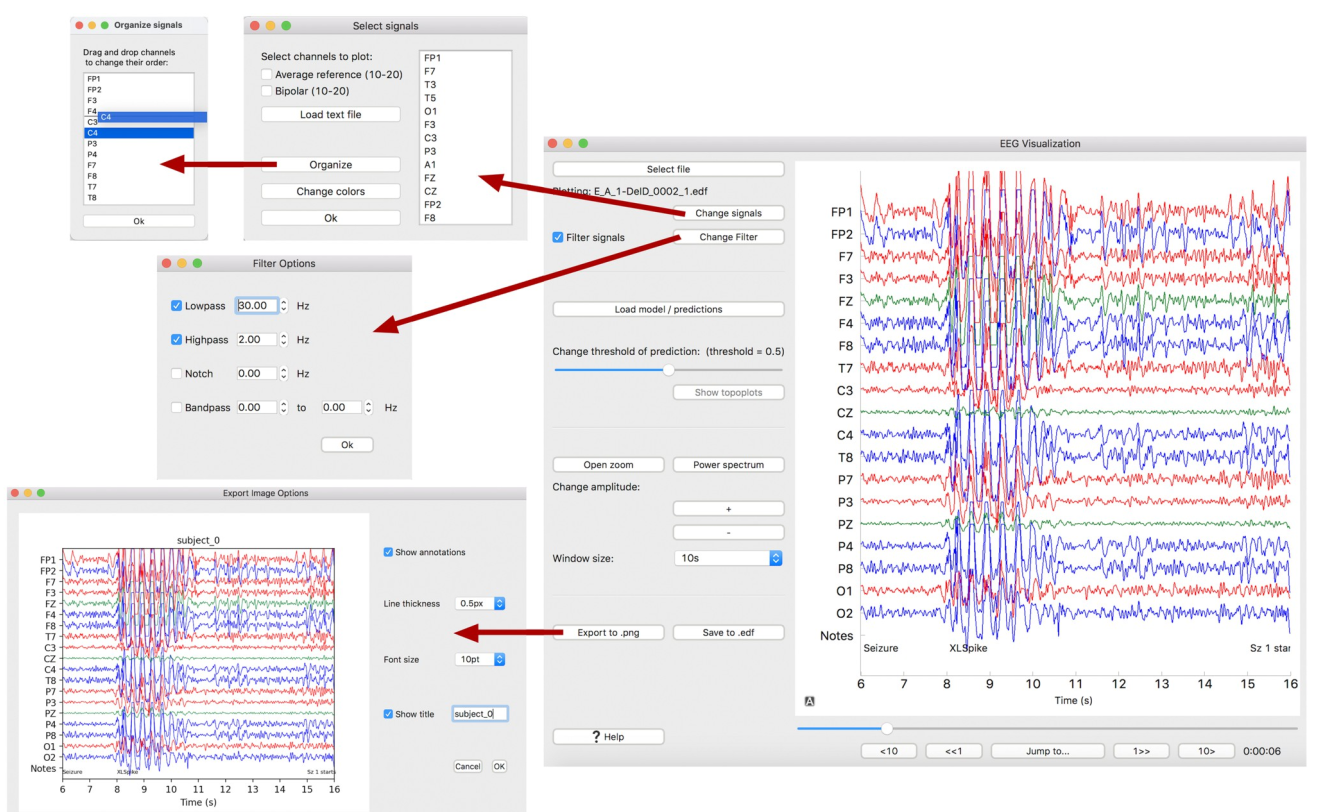
\includegraphics[width=\linewidth]{images/epviz00}
				\caption{EPviz - Visualização por gráficos de linhas}
				\label{fig:epviz00}
			\end{figure}
		\end{column}
		\begin{column}{0.3\textwidth}
			\par A visualização por linhas é eficiente pois nela fica claro os componentes de alta e baixa frequência. No exemplo ao lado o programa EPViz visualiza os sinais captados por todos os eletrodos fornecendo uma boa visão geral. No entanto falta a visão em detalhe que permitiria uma análise mais exata das curvas mostradas.
		\end{column}
	\end{columns}
\end{frame}
\begin{frame}
	\frametitle{Visualização usada em \cite{9098189}}
	\begin{columns}
		\begin{column}{0.5\textwidth}
			\begin{figure}
				\centering
				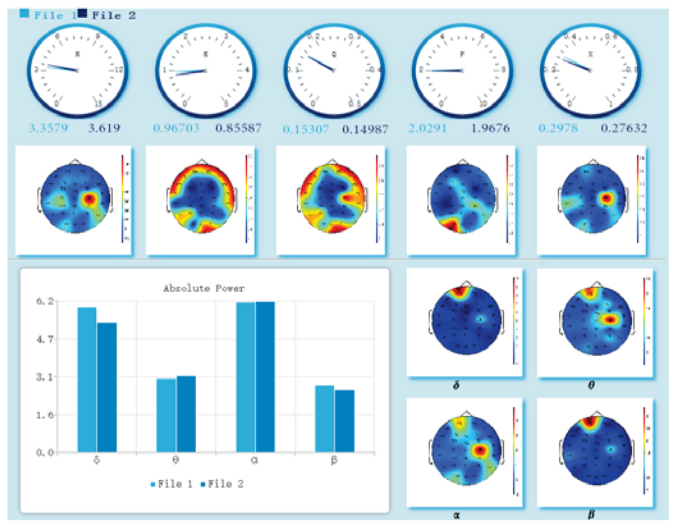
\includegraphics[width=\linewidth]{images/visu01}
				\caption{Visualização topológica}
				\label{fig:visu01}
			\end{figure}
		\end{column}
		\begin{column}{0.5\textwidth}
			\par A metodologia mostrada neste trabalho usa mapas topológicos de cores para indicar a energia do sinal em cada sensor, dessa forma é possível ver as regiões do cérebro com atividade mais intensa no tempo do sinal correspondente, também é interessante a marcação dos identificadores de cada sensor, no entanto, a visualização faz uma interpolação dos valores medidos levando a uma interpretação não necessariamente verdadeira de que as intensidades variam segundo gradientes. 
		\end{column}
	\end{columns}
\end{frame}
\begin{frame}
	\frametitle{Visualização usada em \cite{8937083}}
	\begin{columns}
		\begin{column}{0.6	\textwidth}
			\par Aqui novamente o problema do gradiente ocorre, porém é importante notar a simplificação na visualização que mostra o estado da atividade cerebral em quatro diferentes momentos do cérebro.
		\end{column}
		\begin{column}{0.4\textwidth}
			\begin{figure}
				\centering
				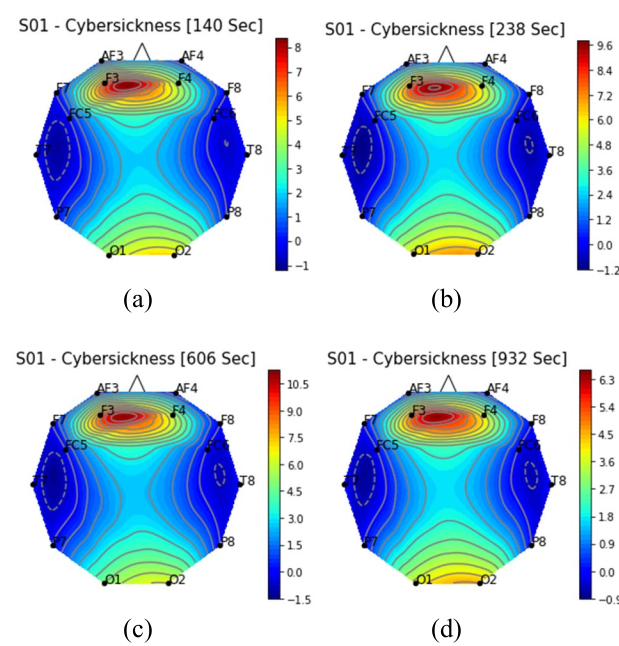
\includegraphics[width=\linewidth]{images/visu02}
				\caption{Visualização topológica}
				\label{fig:visu02}
			\end{figure}
		\end{column}
	\end{columns}
	
\end{frame}